\documentclass[a4page, twocolumn, twoside, 11pt]{article}

\usepackage[utf8]{inputenc}

\usepackage[top=2cm, bottom=2cm, left=1cm, right=1cm]{geometry}

\usepackage{cmbright}
\usepackage{microtype}
\usepackage[none]{hyphenat}

\usepackage[colorlinks, allcolors=blue]{hyperref}

\usepackage{tikz}

\usepackage{amsmath}

\usepackage[noabbrev, capitalise]{cleveref}

\title{Finite Difference of the 1D Explicit Heat Equation}
\author{Dr J.\ A.\ Gopsill}
\date{2019}

\begin{document}

\maketitle

%\section{Introduction}

The one-dimensional transient heat conduction equation without heat generating sources is given by:

\begin{equation}
  \rho c_p \frac{\partial T}{\partial t} = \frac{\partial}{\partial x}\left(k\frac{\partial T}{\partial x}\right)
\end{equation}

\noindent where $\rho$ is the density, $c_p$ heat capacity, $k$ thermal conductivity, $T$ temperature, $x$ distance, and $t$ time.

If $\rho$, $c_p$ and $k$ are constant then the equation can be simplified to:

\begin{equation}
  \frac{\partial T}{\partial t} = \kappa\frac{\partial^2 T}{\partial x^2}
  \label{equ:1d-equation}
\end{equation}

\noindent where:

\begin{equation}
  \kappa = \frac{k}{\rho c_p}
\end{equation}

Examples of the heat equation being used in practice is where a thin body with thermal conductivity $\kappa$ (e.g.\ rod or laminate) is at a starting temperature of $T_s$, is heated at both ends at a constant temperature $T_b$ and insulated along its length $L$ so there is no heating along the orthogonal axes (\cref{fig:model}). In this situation, one might be interested in how long it will take for the body to reach $T_b$.

\begin{figure}
  \centering
  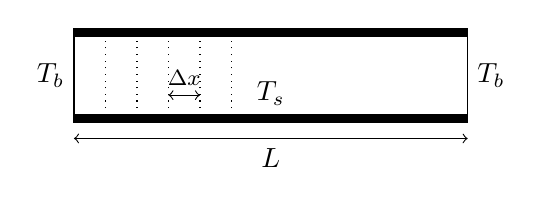
\begin{tikzpicture}
    \draw[] (0,0) -- (5,0) node[pos=0.5, anchor=south] {$T_s$} -- (5,1) node[pos=0.5, anchor=west] {$T_b$} -- (0,1) -- (0,0) node[pos=0.5, anchor=east] {$T_b$};

    \draw[fill] (0,0) -- (5,0) -- (5,-0.1) -- (0,-0.1) -- (0,0);
    \draw[fill] (0,1) -- (5,1) -- (5,1.1) -- (0,1.1) -- (0,0);

    \draw[<->] (0,-0.3) -- (5,-0.3) node[pos=0.5, anchor=north] {$L$};

    \draw[dotted] (0.4,0) -- (0.4,1);
    \draw[dotted] (0.8,0) -- (0.8,1);
    \draw[dotted] (1.2,0) -- (1.2,1);
    \draw[<->] (1.2, 0.25) -- (1.6, 0.25) node[pos=0.5, anchor=south] {\footnotesize $\Delta x$};
    \draw[dotted] (1.6,0) -- (1.6,1);
    \draw[dotted] (2.0,0) -- (2.0,1);
  \end{tikzpicture}
  \caption{1D Heat Model}\label{fig:model}
\end{figure}

We cen solve this numerically be discretising the continuous derivatives ($\partial t, \partial x$) in \cref{equ:1d-equation} using finite difference methods. Lets first look at the time derivative $\frac{\partial T}{\partial t}$, which can be approximated using the forward finite difference approximation.

\begin{equation}
  \frac{\partial T}{\partial t} \approx \frac{ T^{n+1}_{i}-T^{n}_{i} }{ T^{n+1}-t^{n} } = \frac{ T^{n+1}_{i}-T^{n}_{i} }{ \Delta t }
  \label{equ:forward}
\end{equation}

\noindent where $n$ is a step in time and $i$ is a point along the discretised domain.

Second, we turn our attention to the spatial derivative $\frac{\partial^2 T}{\partial x^2}$, which and be approximated using central difference approximation.

\begin{equation}
  \begin{split}
    \frac{\partial T}{\partial x^2} = \frac{\partial}{\partial x}\left(\frac{\partial T}{\partial x}\right) & \approx \frac{ \frac{ T^{n}_{i+1}-T^{n}_{i} }{ \Delta x } - \frac{ T^{n}_{i}-T^{n}_{i-1} }{ \Delta x } }{\Delta x} \\ & \approx \frac{T^n_{i+1}-2T^n_i+T^n_{i-1}}{\Delta x^2}
  \end{split}
  \label{equ:central}
\end{equation}

Substituting \cref{equ:forward,equ:central} into \cref{equ:1d-equation} gives:

\begin{equation}
  \frac{T^{n+1}_{i}-T^{n}_{i}}{\Delta t} = \kappa \left(\frac{T^n_{i+1}-2T^n_i+T^n_{i-1}}{\Delta x^2}\right)
\end{equation}

Rearranging for $T^{n+1}_{i}$ gives:

\begin{equation}
  T^{n+1}_{i} = T^{n}_{i} + \kappa\Delta t \left(\frac{T^n_{i+1}-2T^n_i+T^n_{i-1}}{\Delta x^2}\right)
\end{equation}


\end{document}